\documentclass[a4paper]{report}
\usepackage[utf8]{inputenc}
\usepackage[portuguese]{babel}
\usepackage{hyperref}
\usepackage{a4wide}
\hypersetup{pdftitle={AA},
pdfauthor={João Teixeira, José Ferreira},
colorlinks=true,
urlcolor=blue,
linkcolor=black}
\usepackage{subcaption}
\usepackage[cache=false]{minted}
\usepackage{listings}
\usepackage{booktabs}
\usepackage{multirow}
\usepackage{appendix}
\usepackage{tikz}
\usepackage{authblk}
\usepackage{bashful}
\usepackage{verbatim}
\usepackage{amssymb}
\usepackage{multirow}
\usepackage{mwe}
\usepackage[parfill]{parskip}
\usetikzlibrary{positioning,automata,decorations.markings}
\AfterEndEnvironment{figure}{\noindent\ignorespaces}
\AfterEndEnvironment{table}{\noindent\ignorespaces}

\begin{document}

\title{Advanced Architectures\\Matrix-matrix multiplication}
\author{João Teixeira (A85504) \and José Filipe Ferreira (A83683)}
\date{\today}

\begin{center}
    \begin{minipage}{0.75\linewidth}
        \centering
        
\includegraphics[width=0.4\textwidth]{images/eng.jpeg}\par\vspace{1cm}
        \vspace{1.5cm}
        \href{https://www.uminho.pt/PT}
        {\color{black}{\scshape\LARGE Universidade do Minho}} \par
        \vspace{1cm}
        \href{https://www.di.uminho.pt/}
        {\color{black}{\scshape\Large Departamento de Informática}} \par
        \vspace{1.5cm}
        \maketitle
    \end{minipage}
\end{center}

\tableofcontents

\pagebreak

\chapter{Introduction}

\chapter{Full characterization of the hardware platform}
Our team's main laptop is a Lenovo ThinkPad X260. It is powered by a i5-6300U, a
dual-core hyperthreaded skylake cpu.

To get more information related to the CPU's memory hierarchy we used the
command \textit{lstopo} that displays a graphic with information related with
the cache size.
\begin{figure}[H]
    \centering
        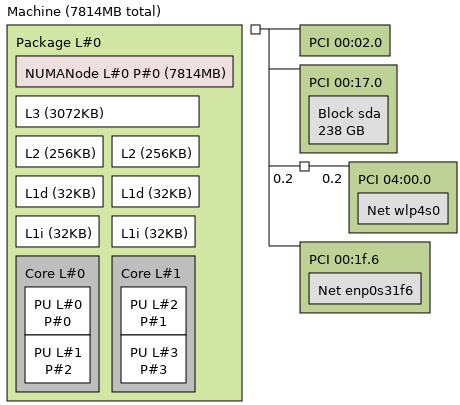
\includegraphics[width=0.6\textwidth]{images/lstopo.png}
        \caption{lstopo output}
\end{figure}

As it is visible in the picture above the cpu has 32KiB L1 cache per core,
256KiB per core and 3072MiB L3 cache. It also has 7814MiB of Random Access
Memory(RAM).

\chapter{Performance of different matrix multiplication algorithms \& implementations}

\chapter{Conclusions}



\end{document}
